\section{Experimental Results
\label{sec:exp_results}}


\begin{table}
\caption{Properties of the outer valence spectra of mixed ArXe clusters. 
Spectra of pure Ar and Xe clusters are included for reference. 
All spectra were recorded at $h\nu = 17$~eV, except for the pure Xe clusters ($h\nu = 60$~eV). 
Binding energies $\EB$ were determined as the centre of gravity of the respective feature, while band width $w$ are the FWHM of a Gaussian fit. 
The average Xe content of the cluster ensemble, Xe$_{\rm cl}$, was determined from the areas of the respective photolines, corrected by their atomic photoionization cross sections (Ar 33.0 Mb, Xe 51.3 Mb)\cite{samson2002}.
Uncertainties are estimated as $\pm$3\,\% for the Xe content and 0.05~eV for the binding energies. 
For reference, the row labelled `(th.)' gives the binding energies used in the simulations of this paper (same as in Ref. \citenum{Fasshauer13}), and the last row their atomic counterparts. 
Values for Ar 3p in these two rows refer to the fine structure states.
\label{tab:valence} }
\begin{tabular}{ l c c c c c c c c}
%
\toprule
 \multicolumn{2}{r}{size} &  Xe$_{in}$& $\EB$ (eV)& $w$ (eV)& \multicolumn{2}{c}{$\EB$ (eV)}  & $w$ (eV) &  Xe$_{\rm cl}$ \\
%
 \multicolumn{2}{r}{(label)}&  (\%) & Ar 3p & Ar 3p & Xe 5p$_{1/2}$ &  Xe 5p$_{3/2}$ & Xe 5p$_{3/2}$  &  (\%) \\
\midrule
% Ar, from Marko
 Ar & (1) &&  15.3  &  1.1 & & & &  \\
% Ar, from Marko 
 Ar & (2) &&  15.1  &  1.3 & & & &  \\
%
%  columns in the following: energies c.g. 51-plt-oval, widths Marko Diss., Xe content Marko Diss
% 1103 676, 679
 ArXe & S &1.2 & 15.36 & 0.9 & 13.07 & 11.75 & 0.85 & 12\\
% 1103 670
 ArXe & M &1.2 & 15.30 & 1.0 & 12.97 & 11.61 & 0.85 & 11\\
% 1103 671
 ArXe & L &1.2 & 15.25 & 1.1 & 12.91 & 11.52 & 1.08 & 10\\
% 1103 663
 ArXe & S &3.0 & 15.39 & 0.8 & 13.06 & 11.68 & 1.02 & 29\\
% 1103 640
 ArXe & M &5.0 & 15.31 & 0.6 & 12.96 & 11.44 & 1.24 & 53\\
% 0506 
 Xe &  & & & & 12.76 & 11.19 & 1.18 & 100\\
%
\midrule
%
%  1004  886  (UHe, c.g. + roi values)
 ArXe & XL &2.5 & 15.15 & 1.3 & 12.59 & 11.01 & 1.24 & 19\\
%
\midrule
%
 Ar, Xe & (th.) && 14.76|15.54 && 12.53 & 10.83 &&\\
%
 \multicolumn{2}{l}{(atomic)\cite{velchev,sansonetti}} && 15.76|15.94 && 13.43 & 12.13 &&\\
%
\bottomrule
\end{tabular}
\end{table}

\subsection{Outer valence spectra}
%
\begin{figure}[ht]
 \centering
 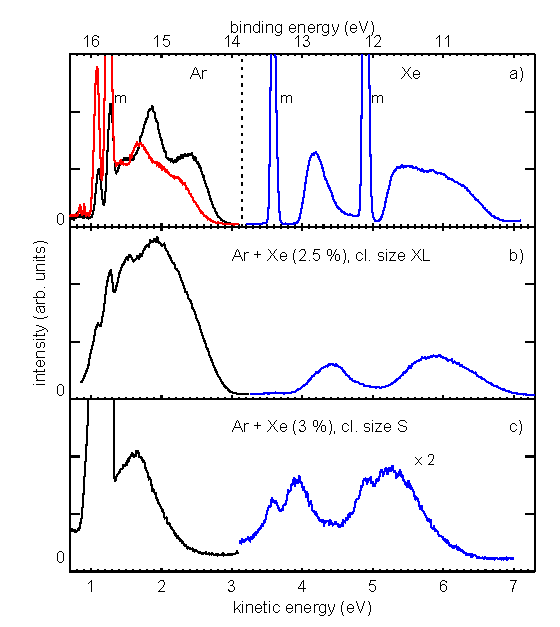
\includegraphics[width=8.5cm]{pics/figure_oval_1.pdf}
 \caption{
Outer valence photoelectron spectra of mixed Ar-Xe clusters, in comparison to the pure species. 
(a) shows the outer valence region of homogeneous Ar and Xe clusters, respectively (see text for details). 
The two lower panels show spectra of the mixed species with different mean size. 
Sharp lines marked `m' result from photoionization of uncondensed atoms into the Ar 3p$_{1/2,3/2}$ and Xe 5p$_{1/2,3/2}$ final states. 
Labels in (b) and (c) give the Xe content in the expanding gas mixture (Xe$_{\rm in}$), which is lower then the Xe content observed in the heterogeneous clusters (Xe$_{\rm cl}$). 
The photon energy was 17~eV, apart from the pure Xe cluster spectrum (60 eV).
}
 \label{figure:oval1}
\end{figure}


\begin{figure}[ht]
 \centering
 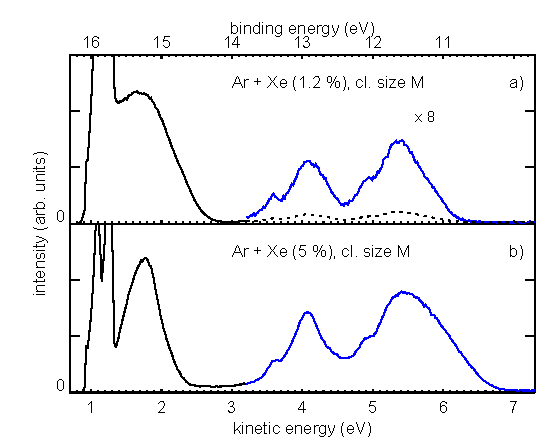
\includegraphics[width=8.5cm]{pics/figure_oval_2.pdf}
 \caption{
Outer valence photoelectron spectra of mixed Ar-Xe clusters from gas mixtures with different Xe concentration. 
For better visibility, a scaling factor is applied to the Xe part of the spectrum in (a).
See Fig.\ \ref{figure:oval1} and text for details.
}
 \label{figure:oval2}
\end{figure}

Figure \ref{figure:oval1} shows the outer valence spectra of small and large ArXe clusters, compared to clusters of the pure gases. 
Qualitatively similar spectra have been published without detailed discussion in Ref.\ \citenum{lindblad}.
Differences are seen in particular for the Ar component. 
In pure Ar clusters, outer valence photoionization leads to a broad band, caused both by spin-orbit coupling and crystal field splitting. 
The relative importance of these two mechanisms remains under debate.\cite{hergenhahnprb,rolles,foerstel_arg1_2010} 
For larger clusters (e.g. $\langle N\rangle = 190$, black trace), the maximum at low binding energies becomes more pronounced, and is identified with emission from the cluster interior.\cite{hergenhahnprb,rolles}
At the particular photon energy selected here, atop of this band a sharp feature is also visible (in Figure \ref{figure:oval1} at a kinetic energy of about 1.8 eV). 
For larger clusters (above $\langle N\rangle \approx 100$), it shows a dispersion characteristic for photoemission of crystalline bulk matter.\cite{foerstel_arg1_2010,foerstel_arg2_2011} 

Ar 3p spectra of the mixed clusters show neither of these traits.
Rather, the Ar band is symmetric, less wide than in the pure clusters and at a higher binding energy. 
For further interpretation of the shape we refer to photoemission spectra of condensed Ar monolayers, measured in several settings.\cite{jacobi,jacobi2}
Spectra were reported for physisorption of Ar on two different metal single crystal substrates, and for Ar atop of a Xe spacer layer adsorbed on the metal.
While the binding energy is substrate dependent, the spectral shape is very similar in all cases. 
Most spectra were recorded for emission along the surface normal, and show a double peak split by about 0.5 eV, leading to a structure with $w$ about 1 eV.
Although this value is larger than the gas phase fine structure split of 0.18 eV, the pertaining states have been assigned to Ar 3p$_{1/2}$ and 3p$_{3/2}$.
A crystal field splitting of the 3p$_{3/2}$ state is assumed to be also present, but with a smaller value of 0.1-0.2 eV, approx.\cite{jacobi2} 
The spectrum changes drastically when going to an angle of 40$^\circ$ with respect to the surface normal (Fig. 2 in Ref.\ \citenum{jacobi2}).
The higher binding energy peak significantly loses in intensity, and the spectrum is now dominated by a single peak comprising both crystal field split substates of Ar 3p$_{3/2}$, with a $w$ of only 0.4 eV.
As our clusters are probed under all angles at the same time, grazing emission will be the rule, and thus we consider the comparison to a thin Ar layer to be satisfactory. 
The larger value of the widths measured in our experiments is believed to result from the implicit averaging over several emission directions.

Emission from the Xe 5p state shows a much larger fine structure splitting, which dominates the spectrum even in clusters (where other broadening mechanisms are also present). 
For the mixed clusters, the Xe band broadens and shifts towards lower binding energy for larger size clusters. 
For pure Xe clusters, an asymmetry observed in the Xe 5p$_{3/2}$ part has no counterpart in the respective spectra from the mixed clusters.
This might be caused by the difference in photon energy, as can be seen from a comparison to literature spectra (ArXe at $h\nu = 90$ eV in Ref.\ \citenum{lindblad}, Xe at $h\nu = 20$ eV in Ref.\ \citenum{rolles}).
For the largest clusters, the nominal size yielded from the jet parameters applied to a pure Xe expansion would correspond to clusters in which bulk atoms far outweigh those on the surface.
At least for the 5p$_{1/2}$, this would be a seen as a clear asymmetry towards the low binding energy side, which is not observed in our spectra.

In Figure \ref{figure:oval2}, we compare the outer valence spectra of clusters with similar expansion conditions, but different composition of the gas mixture.
A Xe-rich mixture obviously leads to clusters with more intense Xe photolines, but besides that the main change consists in a narrowing of the Ar band, which remains at about the same binding energy though.
A comparison with the Ar monomer features (clipped in the Figure) also shows an increased degree of condensation for the Ar gas in the expansion.
Finally, comparing Figure \ref{figure:oval2} to \ref{figure:oval1} reveals that much larger changes in the valence emission spectra occur for changes in the expansion conditions than for changes of the gax mixture.
This finding is supported by the spectra shown in Ref.\ \citenum{lindblad}.
%
%
\subsection{Inner valence and electron-electron coincidence spectra}
%
\begin{figure}[ht]
 \centering
 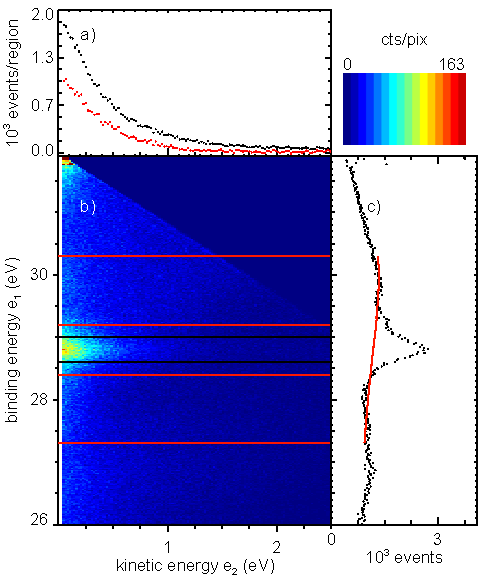
\includegraphics[width=8.5cm]{pics/figure_map.pdf}
 \caption{
Photon excited electron-electron coincidence spectrum of mixed Ar-Xe clusters in the inner valence region. 
(b): Color-coded map of coincident electron pairs, with the electron of higher kinetic named $e_1$. 
The energy of $e_1$ is given as binding energy, using the photon energy of $h\nu = 32$~eV. 
(c): Energy spectrum of primary electrons $e_1$, irrespective of the energy of the secondary electron (summation of the coincidence map along horizontal lines). 
(a): Energy spectrum of all secondary (ICD or ETMD) electrons $e_2$ pertaining to the Ar 3s binding energy region marked by two black bars. 
See text for details. 
Intensity is expressed as coincident events/pixel of 20~meV$^2$ (b) or as coincident events per interval of 20~meV (a,c). 
In total, approx. 4$\times 10^5$ events are shown. 
The color scale of (b) is linear.
 \label{figure:map}
 }
\end{figure}
%
In our system, only inner valence and core ionized states have sufficient energy to decay via ICD. 
Here, we focus on the Ar inner valence (3s) vacancy states. 
Figure\ \ref{figure:map}b shows a typical electron-electron coincidence spectrum pertaining to primary ionization of energy levels in the inner valence region of binding energies.
More conventional, one-dimensional electron spectra pertaining to the photoelectrons and the ICD/ETMD electrons are obtained by summing up along one of the energy axis of the two-dimensional map, and are shown in (c) and (a). 
The peak in Figure \ref{figure:map}c at a binding energy of 28.7~eV pertains to the Ar 3s photoelectron line.
No atomic counterpart of this line is visible in this Figure, as only the cluster photoelectrons lead to electron-electron coincidences (see below).
The Figure shows that a significant amount of slow electrons $e_2$ are recorded in coincidence with the primary 3s electrons ($e_1$), which have a kinetic energy of approx. 3.3 eV. 
Some background of electron pairs at other energies is also visible.
This results from inelastic scattering of outer valence photoelectrons, and (in particular for the feature which has both electrons with kinetic energy less than 0.2 eV, upper left corner of \ref{figure:map}b) due to inelastic scattering at parts of the analyzer.
We subtract this background by fitting a second order polynomial to the background, marked by the two pairs of red horizontal bars, and subtract it from ICD/ETMD signal between the pair of black bars.
A different polynomial is used for each 0.5 eV wide interval of $e_2$ energies.
The summation of all background signals is shown as a wavy, solid line in Figure \ref{figure:map}c, and the signal of secondary electron, background subtracted, is shown as the lower trace of data points in Figure \ref{figure:map}a.
These data were recorded under all expansion conditions listed in Table\ \ref{tab:cluster}.

\begin{figure}[ht]
 \centering
 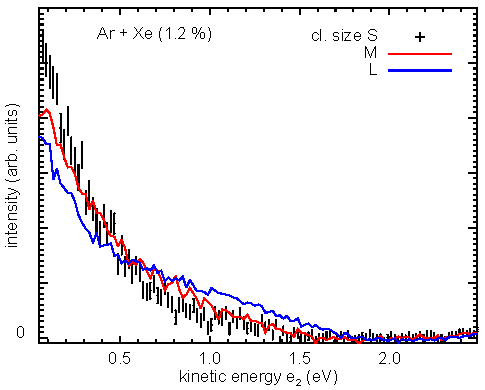
\includegraphics[width=8.5cm]{pics/figure_icd_12.pdf}
 \caption{
Energy spectrum of all coincident secondary (ICD or ETMD) electrons $e_2$ pertaining to primary electrons $e_1$ in the Ar 3s binding energy region. Spectra were recorded with a photon energy of $h\nu = 32$~eV. Black symbols with error bars show the data points for the smallest clusters measured (`S'), two larger clusters sizes are shown by the red and blue traces. For comparison, all spectra are shown area-normalized. 
}
 \label{figure:icd_12}
\end{figure}


\begin{figure}[ht]
 \centering
 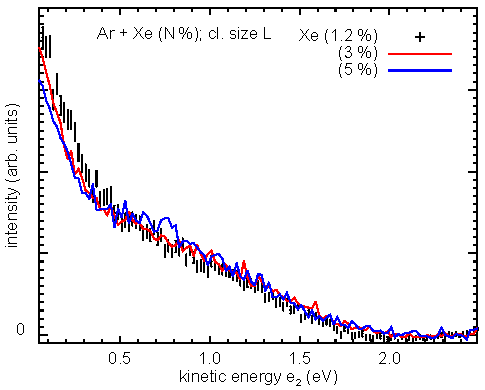
\includegraphics[width=8.5cm]{pics/figure_icd_l.pdf}
 \caption{
Energy spectrum of all coincident secondary (ICD or ETMD) electrons $e_2$ for clusters of the same size, but from gas mixtures with different Xe concentration. See Figure \protect\ref{figure:icd_12} for details.
}
 \label{figure:icd_l}
\end{figure}


\begin{figure}[ht]
 \centering
 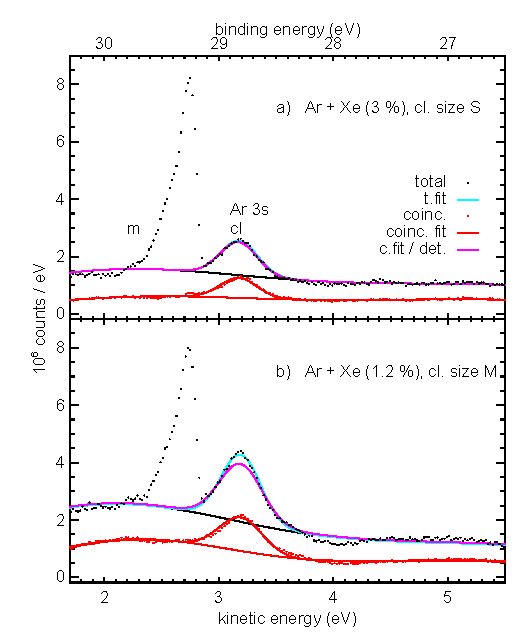
\includegraphics[width=8.5cm]{pics/figure_ival.pdf}
 \caption{
Photon excited electron spectra and electron-electron coincidence spectra of mixed Ar-Xe clusters in the inner valence region. Spectra show the Ar 3s photoline from clusters (`cl') and uncondensed Ar monomers (`m'), atop of a background resulting from inelastic intracluster scattering of outer valence photoelectrons.\protect\cite{hergenhahn2002} Black symbols: sum of non-coincident and coincident (1st hit) events, red symbols: coincident events only. Solid, colored lines show the results of various least-squares fits, see text for details.
}
 \label{figure:ival}
\end{figure}



\begin{figure}[ht]
 \centering
 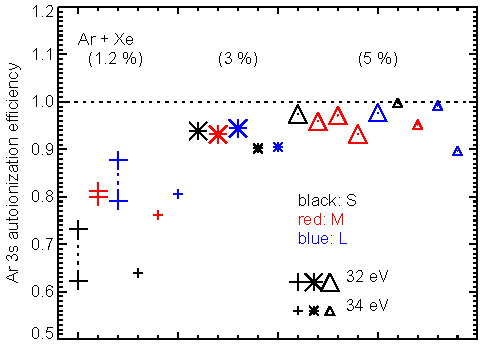
\includegraphics[width=8.5cm]{pics/figure_eff.pdf}
 \caption{
Efficiency of the decay of Ar 3s ionized states in ArXe clusters by emission of a secondary electron via ICD or ETMD. Values are arranged by Xe content of the initial gas mixture ('+' symbols: 1.2\,\%, asterisk: 3\,\%, triangle: 5\,\%). Symbol sizes indicate the photon energy (large symbols: 32 eV, small: 34 eV), and color indicates the cluster size (black symbols: S, red: M, blue: L). See text for details.
}
 \label{figure:eff}
\end{figure}
